% !TEX root = ../ac_paper.tex

\section{Reinforcement Learning}\label{sec:rl}



This section is divided as follows: in \autoref{sec:mdp}, we discuss how the problem underlying Andrews-Curtis conjecture can be modelled as a Markov Decision Process. In \autoref{sec:ppo}, we will discuss some details of a specific reinforcement learning algorithm, called Proximal Policy Optimization algorithm that we used to find AC trivializations of balanced presentations. Finally, in \autoref{sec:application}, we discuss the results of our work, comparing the performance of PPO with that of the classical search algorithms studied in the previous section. 

\subsection{Markov Decision Process} \label{sec:mdp}

A Markov Decision Process (MDP) is a 5-tuple $(S, A, R, P, \rho)$ where 
\begin{itemize}
	\item $S$ is the space of states, 
	\item $A$ is the set of actions, i.e. $a \colon S \to S \ \forall \ a \in A$, 
	\item $R \colon S \times A \times S \to \mathbb{R}$ is the ``reward" function, 
	\item $P \colon S \times A \to \mathcal{P}(S)$ is the transition probability function, and 
	\item $\rho$ is the initial probability distribution of states. 
\end{itemize}

The schematic picture of how these objects interact with each other is as follows. We start with a state $s_0$ sampled from the distribution $\rho$ and take an action $a_0$. This results in a state $s_1$ with probability $P(s_1 \mid s_0, a_0) $. The transition gets a ``reward" $r_0 = R(s_0, a_0, s_1)$ which quantifies the effectiveness of the action in contributing toward achieving an ultimate goal. From state $s_1$, we repeat this process, obtaining a trajectory of states
\[
\tau = \left( s_0, a_0, s_1, a_1, \cdots \right)
\]
The goal of this process is to maximize the cumulative return,
\[
R(\tau) = \sum\limits_{t=0}^{T} \gamma^t R(s_t, a_t, s_{t+1})
\]
Here, $T$ is the length of the trajectory and $\gamma \in \left(0, 1 \right)$ is the ``discount factor" that assigns smaller weights to the reward values obtained farther in the future. 
\newline

For a given problem at hand, we may not \textit{a priori} know the actions $\{a_t\}$ and states $\{s_{t+1}\}$ that maximize the return. Deep reinforcement learning presents a solution to this problem: we train a neural network that learns a map from states to actions with the objective of maximizing the cumulative return. More precisely, we learn a map called the ``policy" function $\pi : S \to \mathcal{P}(A)$ that assigns to each state a probability distribution over actions. At time step $t$, an action $a_t \sim \pi(\cdot \mid s_t)$ is sampled that gives the next state $s_{t+1}$.
\footnote{In general, we need to specify the probability transition function $P(\cdot \mid s_t, a_t)$  from which the next state would be sampled. In this paper, we take this probability distribution to be a delta function centered at a single state, which we write as $a_t(s_t)$.} 
The specific neural network architecture and the objective function we used in this paper is discussed in the next subsection.
\newline 

\subsection{Proximal Policy Optimization} \label{sec:ppo}

The goal of our optimization process is to find a policy that maximizes the cumulative return. The most naive way to achieve this goal is through an algorithm known as the ``vanilla policy gradient" algiorithm. We perform gradient updates guided by the expected return $J(\pi_\theta) \equiv \mathbb{E}_{\tau \sim \pi_\theta} R(\tau)$, where the expectation is over a set of trajectories consisting of states and actions sampled according to our current policy, 
\[
\theta_{k+1} = \theta_k + \nabla_\theta J(\pi_\theta)
\]

It turns out that this update depends on the gradient of the logarithm of the policy function itself and an ``advantage function" \( A^\pi (s, a) \) which quantifies the relative benefit of taking action \( a \) in state \( s \) under policy \( \pi \) \cite{SpinningUp2018}.
\footnote{
Mathematically, the advantage function is the difference between ``on-policy action-value function" $Q^{\pi}(s, a) = \mathbb{E}_{\tau \sim \pi_\theta} [R(\tau) \mid s_0 = s, a_0 = a]$ and the ``on-policy value function", $V^{\pi}(s) = \mathbb{E}_{\tau \sim \pi_\theta} [R(\tau) \mid s_0 = s]$. These functions give an estimate of the cumulative return given that the current state-action pair is $(s, a)$ in the case of $Q^\pi$ and the current state is $s$ in the case of $V^{\pi}$.
\label{ft:advantage}
}
\begin{align*}
	\nabla_\theta J(\pi_\theta) &= \mathbb{E}_{\tau \sim \pi_\theta} \left[ \sum\limits_{t=0}^T \nabla_\theta \log 								\pi_\theta (a_t \mid s_t) A^{\pi_\theta} (s_t, a_t) \right]
\end{align*}
Thus, vanilla policy gradient algorithm amounts to optimizing the objective function, 
\[
L^{PG} = \mathbb{E}_{\tau \sim \pi_\theta} \left[ \sum\limits_{t=0}^T \log 								\pi_\theta (a_t \mid s_t) A^{\pi_\theta} (s_t, a_t) \right].
\]
Though simple, this algorithm has the downside of taking destructively large updates, thus taking the updated policy too far from the current policy.
\newline 

Proximal Policy Optimization (PPO) algorithms seek to make these updates more robust by limiting the extent to which the policy \( \pi \) can change in a single update \cite{schulman2017proximal}.
PPO implements this through an objective function that includes a clipped probability ratio between the new policy \( \pi_\theta \) and the old policy \( \pi_{\text{old}} \), thus constraining the updates within a predefined range. 
\footnote{Do I need to sum over time inside the expectation value? Probably yes, but think about it. Also, I am using the notation $A^{\pi_\theta}$ in the equations above, but here I am using $A_t$. Choose one convention.}
\[
L^{CLIP}(\theta) = \mathbb{E}_{\tau \sim \pi_\theta} \left[ \min(r_t(\theta) A_t, \text{clip}(r_t(\theta), 1 - \epsilon, 1 + \epsilon) A_t) \right]
\]

Here \( r_t(\theta) = \frac{\pi_\theta(a_t | s_t)}{\pi_{\text{old}}(a_t | s_t)} \) represents the probability ratio, and \( \epsilon \) is a small positive constant (commonly set around 0.1 or 0.2) that controls the clipping value. The raw and the clipped ratio ensure that excessively large policy updates are curtailed, making the optimization process more stable.
\newline 

The advantage function is estimated during the optimization process using the Generalized Advantage Estimation method of 
\cite{schulman2018highdimensional}. 
This function requires an estimation of the on-policy value function (c.f. \autoref{ft:advantage}). PPO uses the actor-critic framework to estimate this function, where the ``actor" learns the policy $\pi_\theta$ and the ``critic" learns the value function.
\footnote{
The actor and the critic are sometimes made to share the neural network parameters except the last layer. This reduces the number of trainable parameters and increases stability in training. We experimened with shared as well as independent parameters and observed better performance by keeping the parameters independent.
}
The value loss $L^V$ is the mean squared error between the values for a state as estimated by value network before and after a gradient update.
Lastly, PPO adds entropy $S$ of the action-space distribution to the full loss function to prevent premature convergence to a suboptimal policy. The full loss function is as follows,
\[
L = \mathbb{E}_{\tau \sim \pi_\theta} [L^{CLIP}(\theta) - c_1 L^{V}(\phi) + c_2 S(\pi_\theta)(s_t)]
\]
where $c_1$ and $c_2$ are tunable hyperparameters.

In policy gradient algorithms such as PPO, we alternate between collecting data through the current policy in the ``rollout phase" and updating the policy weights through gradient descent in the ``optimization phase". There are various hyperparameters associated to these phases, which we briefly describe now. The rollout phase involves generating multiple trajectories of the underlying Markov Decision Process in parallel using the current policy function. The hyperparameters of this phase include the number of parallel actors $N$, the length of the trajectory $T$ (c.f. \autoref{sec:mdp}), the discount factor $\gamma$ (c.f. \autoref{sec:mdp}) and a bootstrapping hyperparameter of Generalized Advantage Estimation $\lambda_{\text{GAE}}$. The dataset of $N \times T$ examples collected in this phase is then used update the policy. In each epoch, the dataset is shuffled and split into minibatches before performing gradient descent. The number of epochs and the size of the minibatch are hyperparameters of the optimization process in addition to the optimizer hyperparameters (such as learning rate schedule) and the hyperparameters that define the loss function. We provide the list of hyperparameters we used in  \autoref{app:hyperparameters}.


\subsection{Application to Andrews-Curtis Conjecture} \label{sec:application}

Now we discuss how we use the notions of Markov Decision Process (MDP) and policy gradient algorithms to find a policy that learns to discover AC trivializations for balanced presentations. The set of all balanced presentations of the trivial group with a fixed number of generators and the set of AC transformations, (AC$'$1) - (AC$'$2), play the role of sets $S$ and $A$ in the notation of MDPs (c.f. \autoref{sec:mdp}). The choice of reward function is up to us. We tested a few different reward functions and noticed the following candidate led to high returns and stability in training.
\[
R(s_{t}, a_{t}, s_{t+1}) = 
\begin{cases} 
-\min(10, \ \text{length}(s_{t+1})) & \text{if length}(s_{t+1}) > 2 \\
1000 & \text{otherwise } 
\end{cases}
\]
Here $\text{length}(s_{t+1})$ is the length of the presentation at timestep $t+1$. In words, this reward function assigns -$\text{length}(s_{t+1})$ to encourage the optimization process to reward shorter presentations. However, we noticed that clipping this value at $-10$ led to more stable training. We also assigned a larger reward of 1000 when a trivial balanced presentation was found to encourage the actor network towards prioritizing the action sequence taken in the trajectory. 
\newline

The initial distribution of states $\rho$ of the MDP was chosen to be the following. At the start of the training process, the rollout trajectories were initiated with presentation of the Miller-Schupp series dataset from \autoref{sec:conjecture} in the increasing order of $n$ and $\text{length}(w)$. We continued this until each presentation of the dataset had been chosen exactly once. Afterwards, we randomly selected a presentation that had already been solved in a rollout with probability $\frac{1}{4}$, and a presentation that had so far remained unsolved with probability $\frac{3}{4}$. These choices were made so that the policy continues to learn from and improve its performance on the presentations that had already been solved (finding shorter sequences of AC moves for them if possible) while also attempting to solve the newer presentations. 
\newline

Next, we discuss the results of our experiments which should be understood in the context of some hyperparameter choices we made. 

We made several choices of hyperparameters based on performance and compute constraints. Hence it is necessary to interpret the results in the light of the our choices.

We set the maximum path length at 200. Doubling this path length would need 3x more compute as optimization process takes 2x more compute when we perform gradient updates for only one epoch. There is also a chance that the model will iterate more slowly and hence learn more slowly as it fails much later. We note from figure 3 that this is not very damaging as only 4 out of 533 presentations solved by greedy search were solved in path lengths of more than 200 moves. So we can expect that all of the other 529 presentations should be solved by PPO. However, we found this to not be the case. PPO could solve only 431 presentations. 

With these results, we can expect that PPO will have a hard time solving any of the presentations that greedy search could not solve. 



PPO could solve 431 out of 533 presentations solved by greedy search. It could not solve any of the presentations unsolved by greedy search. It too could solve all $n=1$ presentations and generally found it easier to solve short presentations. For presentations with short GS path lengths, PPO found even shorter paths. However, for presentations with longer GS path lengths, PPO found even longer paths. 

\fixme{Perhaps these should be two different figures.}
\begin{figure}
	\centering
	\begin{subfigure}[b]{0.5\textwidth}
		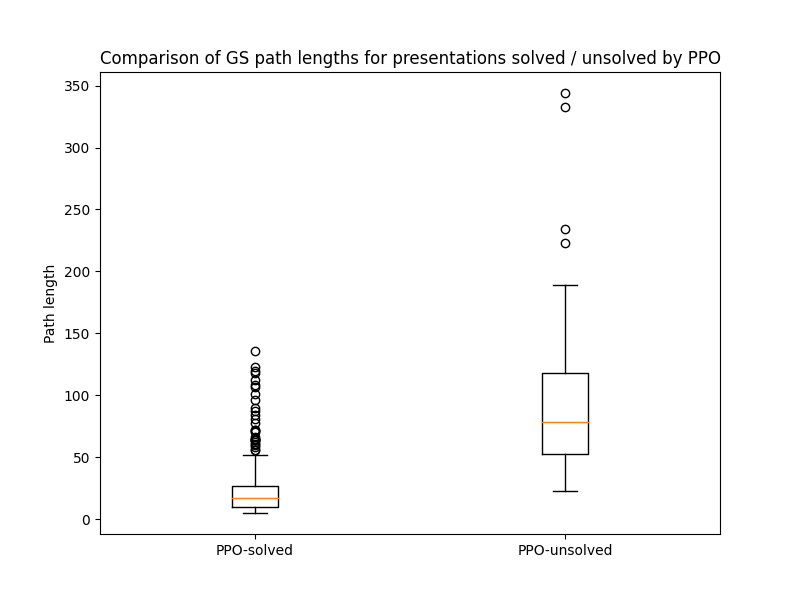
\includegraphics[width=\textwidth]{fig/path_lengths_ppo_solved_vs_unsolved.png}
		\caption{ X}
		%Distribution of path lengths discovered by greedy search for presentations solved / unsolved by Proximal Policy Optimization}
		\label{fig:path_lengths_ppo_solved_vs_unsolved}
	\end{subfigure}%
	%add desired spacing between images, e. g. ~, \quad, \qquad etc.
	%(or a blank line to force the subfigure onto a new line)
	\begin{subfigure}[b]{0.5\textwidth}
		\centering
		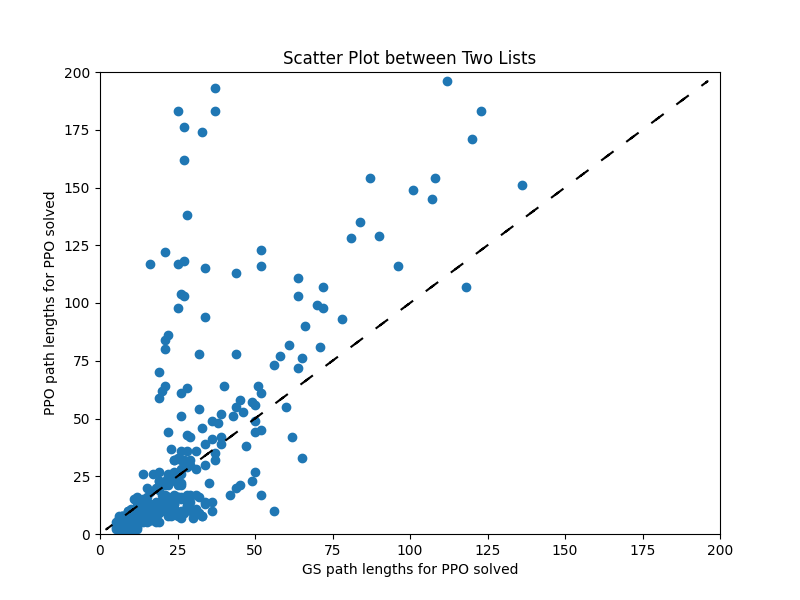
\includegraphics[width=1.1\textwidth]{fig/path_lengths_gs_vs_ppo.png}
		\caption{Scatter plot of path lengths discovered by PPO vs path lengths discovered by greedy search}
		\label{fig:path_lengths_gs_vs_ppo}
	\end{subfigure}
	\caption{
This figure illustrates the maximum increase in the length of a presentation relative to its initial length along the AC trivialization path. The increase is plotted as a function of the initial length of the presentation on the left and as a function of $n$ on the right.} \label{fig:path_lengths_gs_vs_ppo_full}
\end{figure}

\subsection{Supermoves}.

Finally, there exists a notion of "elementary M-transformations" which could be useful \cite{BurnsI, BurnsII}.
Each elementary M-transformation is a composition of AC moves, such that trivializing a presentation requires dramatically less M-transformations compared to the number of AC moves.
For example, trivializing $\AK(2)$ requires 14 AC moves, but only 2 elementary M-transformations.


\subsection{Limitations and further improvements}

Increase path length. Find a way to stably train that. 

It might be useful to try other architectures such as MCTS.

While we did some hyperparameter tuning, the analysis could be done in a much more systematic way. This would require a lot more compute but could be very useful. For example, it will be nice to estimate the critical batch size for optimization. It will also be nice to use the iteration batch-size invariance, i.e. PPO-EWMA so that we can perform our experiments at one iteration batch size. If we get more compute, we can scale the number of parallel actors (wait does iteration batch size tell us about number of parallel actors or horizon length or both?)

We need to strike a balance between the path length and the 

Scale?